\section{Initial Database Architecture}
\subsection{High-Level Architecture Proposal}
\subsection{Entity Relationship Diagram - First Version}
\subsection{Data Flow and Storage Solutions}

Here describes the overall data flow of the platform and the adopted storage solutions. It explains how information moves through the system and how files and metadata are managed across different storage layers.

\begin{figure}[H]
    \centering
    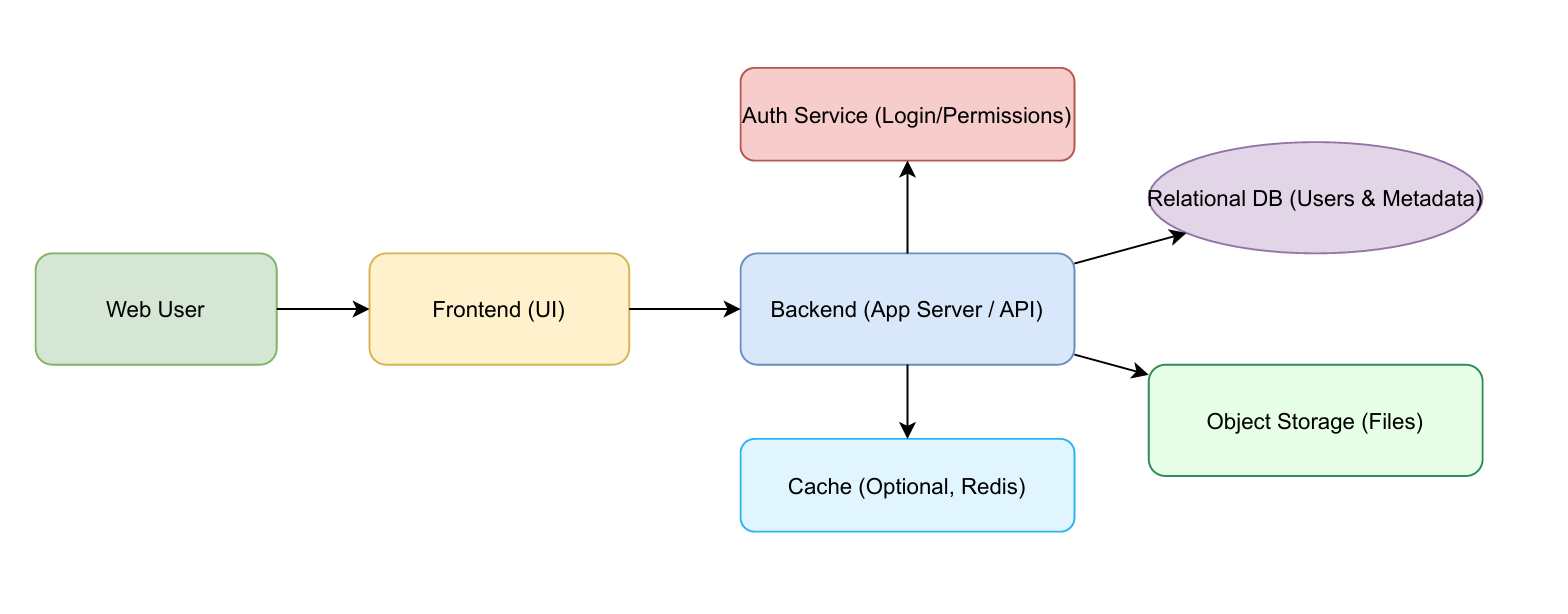
\includegraphics[width=0.95\linewidth,keepaspectratio]{initialdbarch/Dataflow.png}
    \caption{Data Flow and Storage Solutions for the file storage platform.}
    \label{fig:dataflow}
\end{figure}

For the dataflow, it proposed system manages two primary data types: user information and files. The data flow begins when a user interacts with the platform through the web or mobile interface. Requests are sent to the backend application server, which validates user credentials and permissions through the authentication service. Once authenticated, the backend processes the request according to its type:\\

\begin{itemize}
    \item For file uploads, the binary object is stored in the cloud object storage, while metadata, e.g., file name, size, type, upload date, and owner is recorded in the relational database.
    \item For file downloads, the backend verifies user access rights and generates a temporary signed URL, allowing secure file retrieval from the object storage.
    \item For queries such as listing files or browsing folders, the backend retrieves metadata from the database and may leverage a cache layer to accelerate frequent lookups.
\end{itemize}

This flow ensures that every operation is validated, traceable, and optimized for performance while maintaining strict access control. \\

Regarding storage solutions, its design adopts a hybrid model:

\begin{itemize}
    \item Relational Database: like PostgreSQL or MySQL is used for structured information such as user accounts, roles, permissions, and file metadata. This allows enforcing relationships and maintaining consistency.
    \item Object Storage: e.g., AWS S3, Azure Blob is used for binary files, ensuring scalability, durability, and redundancy. This approach allows efficient handling of large files with virtually unlimited capacity.
    \item Cache Layer: for supports faster access to frequently requested metadata, reducing database load.
    \item Backup and Replication strategies: ensure high availability and disaster recovery, minimizing the risk of data loss.
\end{itemize}

This architecture separates file storage from metadata management, providing scalability and flexibility. It also ensures that the platform can handle a growing number of users and files without compromising security, reliability, or performance.
